% Created by tikzDevice version 0.6.2 on 2014-10-03 01:42:39
% !TEX encoding = UTF-8 Unicode
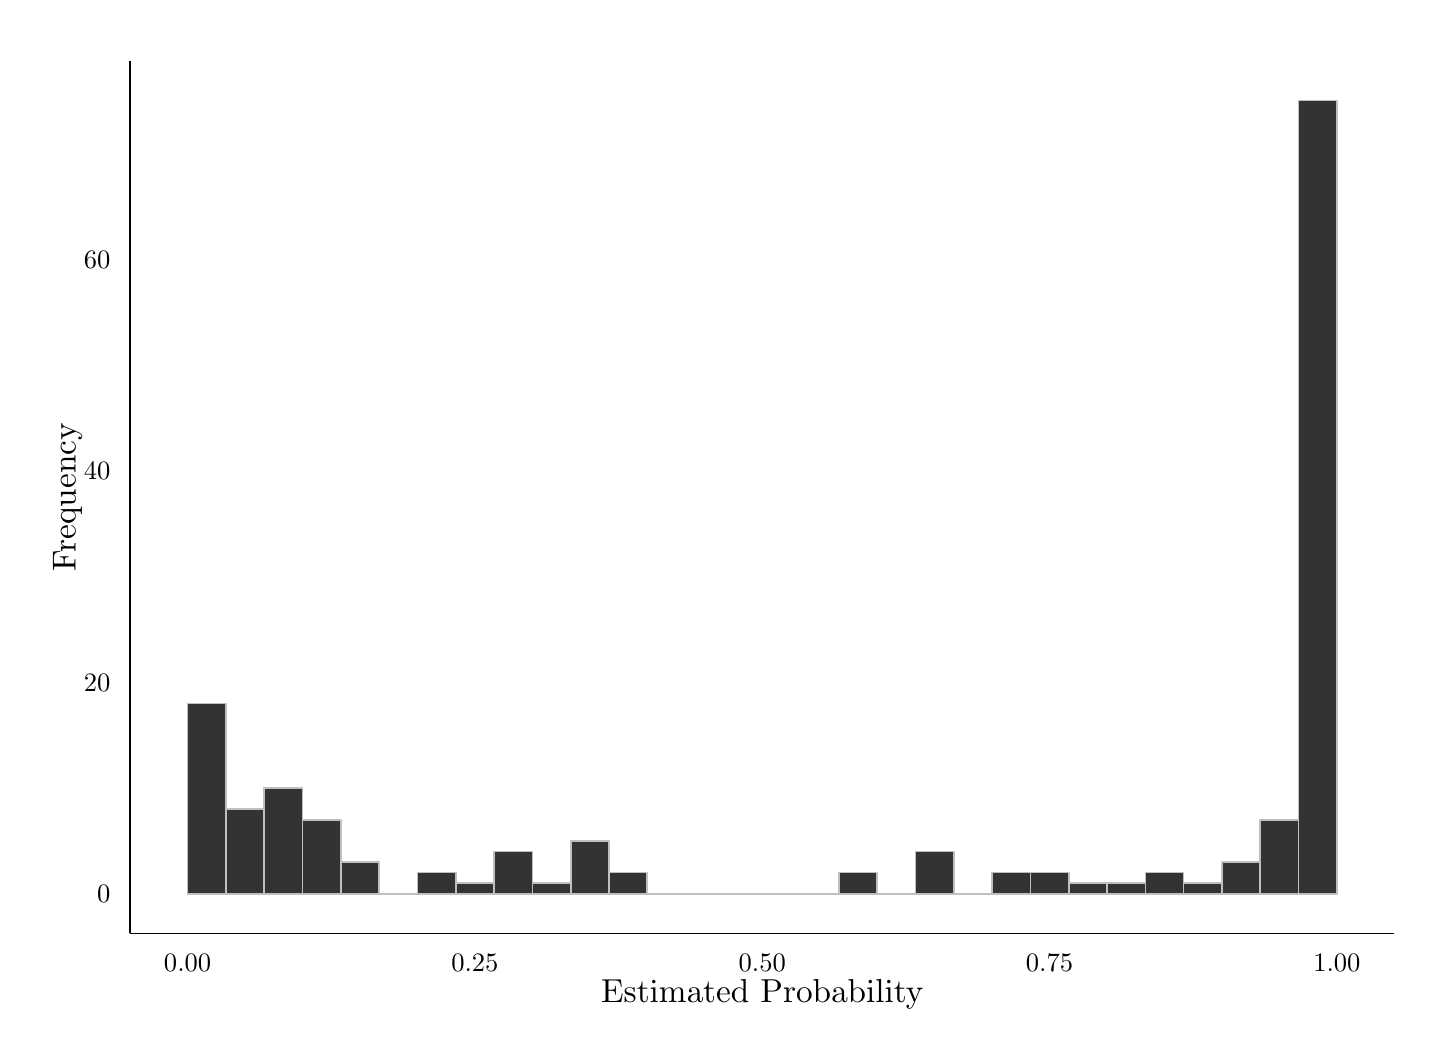
\begin{tikzpicture}[x=1pt,y=1pt]
\definecolor[named]{drawColor}{rgb}{0.00,0.00,0.00}
\definecolor[named]{fillColor}{rgb}{1.00,1.00,1.00}
\fill[color=fillColor,fill opacity=0.00,] (0,0) rectangle (505.89,361.35);
\begin{scope}
\path[clip] (  0.00,  0.00) rectangle (505.89,361.35);
\end{scope}
\begin{scope}
\path[clip] (  0.00,  0.00) rectangle (505.89,361.35);
\end{scope}
\begin{scope}
\path[clip] (  0.00,  0.00) rectangle (505.89,361.35);
\definecolor[named]{drawColor}{rgb}{1.00,1.00,1.00}
\definecolor[named]{fillColor}{rgb}{1.00,1.00,1.00}

\draw[color=drawColor,line width= 0.6pt,line cap=round,line join=round,fill=fillColor,] (  0.00,  0.00) rectangle (505.89,361.35);
\end{scope}
\begin{scope}
\path[clip] (  0.00,  0.00) rectangle (505.89,361.35);
\end{scope}
\begin{scope}
\path[clip] (  0.00,  0.00) rectangle (505.89,361.35);
\end{scope}
\begin{scope}
\path[clip] (  0.00,  0.00) rectangle (505.89,361.35);
\end{scope}
\begin{scope}
\path[clip] ( 37.02, 34.03) rectangle (493.85,349.30);
\definecolor[named]{fillColor}{rgb}{1.00,1.00,1.00}

\draw[fill=fillColor,draw opacity=0.00,] ( 37.02, 34.03) rectangle (493.85,349.30);
\definecolor[named]{drawColor}{rgb}{0.75,0.75,0.75}
\definecolor[named]{fillColor}{rgb}{0.20,0.20,0.20}

\draw[color=drawColor,line width= 0.6pt,line join=round,fill=fillColor,] ( 57.79, 48.37) rectangle ( 71.63,117.15);

\draw[color=drawColor,line width= 0.6pt,line join=round,fill=fillColor,] ( 71.63, 48.37) rectangle ( 85.47, 78.94);

\draw[color=drawColor,line width= 0.6pt,line join=round,fill=fillColor,] ( 85.47, 48.37) rectangle ( 99.31, 86.58);

\draw[color=drawColor,line width= 0.6pt,line join=round,fill=fillColor,] ( 99.31, 48.37) rectangle (113.16, 75.12);

\draw[color=drawColor,line width= 0.6pt,line join=round,fill=fillColor,] (113.16, 48.37) rectangle (127.00, 59.83);

\draw[color=drawColor,line width= 0.6pt,line join=round,fill=fillColor,] (127.00, 48.37) rectangle (140.84, 48.37);

\draw[color=drawColor,line width= 0.6pt,line join=round,fill=fillColor,] (140.84, 48.37) rectangle (154.69, 56.01);

\draw[color=drawColor,line width= 0.6pt,line join=round,fill=fillColor,] (154.69, 48.37) rectangle (168.53, 52.19);

\draw[color=drawColor,line width= 0.6pt,line join=round,fill=fillColor,] (168.53, 48.37) rectangle (182.37, 63.65);

\draw[color=drawColor,line width= 0.6pt,line join=round,fill=fillColor,] (182.37, 48.37) rectangle (196.22, 52.19);

\draw[color=drawColor,line width= 0.6pt,line join=round,fill=fillColor,] (196.22, 48.37) rectangle (210.06, 67.47);

\draw[color=drawColor,line width= 0.6pt,line join=round,fill=fillColor,] (210.06, 48.37) rectangle (223.90, 56.01);

\draw[color=drawColor,line width= 0.6pt,line join=round,fill=fillColor,] (223.90, 48.37) rectangle (237.75, 48.37);

\draw[color=drawColor,line width= 0.6pt,line join=round,fill=fillColor,] (237.75, 48.37) rectangle (251.59, 48.37);

\draw[color=drawColor,line width= 0.6pt,line join=round,fill=fillColor,] (251.59, 48.37) rectangle (265.43, 48.37);

\draw[color=drawColor,line width= 0.6pt,line join=round,fill=fillColor,] (265.43, 48.37) rectangle (279.28, 48.37);

\draw[color=drawColor,line width= 0.6pt,line join=round,fill=fillColor,] (279.28, 48.37) rectangle (293.12, 48.37);

\draw[color=drawColor,line width= 0.6pt,line join=round,fill=fillColor,] (293.12, 48.37) rectangle (306.96, 56.01);

\draw[color=drawColor,line width= 0.6pt,line join=round,fill=fillColor,] (306.96, 48.37) rectangle (320.81, 48.37);

\draw[color=drawColor,line width= 0.6pt,line join=round,fill=fillColor,] (320.81, 48.37) rectangle (334.65, 63.65);

\draw[color=drawColor,line width= 0.6pt,line join=round,fill=fillColor,] (334.65, 48.37) rectangle (348.49, 48.37);

\draw[color=drawColor,line width= 0.6pt,line join=round,fill=fillColor,] (348.49, 48.37) rectangle (362.33, 56.01);

\draw[color=drawColor,line width= 0.6pt,line join=round,fill=fillColor,] (362.33, 48.37) rectangle (376.18, 56.01);

\draw[color=drawColor,line width= 0.6pt,line join=round,fill=fillColor,] (376.18, 48.37) rectangle (390.02, 52.19);

\draw[color=drawColor,line width= 0.6pt,line join=round,fill=fillColor,] (390.02, 48.37) rectangle (403.86, 52.19);

\draw[color=drawColor,line width= 0.6pt,line join=round,fill=fillColor,] (403.86, 48.37) rectangle (417.71, 56.01);

\draw[color=drawColor,line width= 0.6pt,line join=round,fill=fillColor,] (417.71, 48.37) rectangle (431.55, 52.19);

\draw[color=drawColor,line width= 0.6pt,line join=round,fill=fillColor,] (431.55, 48.37) rectangle (445.39, 59.83);

\draw[color=drawColor,line width= 0.6pt,line join=round,fill=fillColor,] (445.39, 48.37) rectangle (459.24, 75.12);

\draw[color=drawColor,line width= 0.6pt,line join=round,fill=fillColor,] (459.24, 48.37) rectangle (473.08,334.97);
\end{scope}
\begin{scope}
\path[clip] (  0.00,  0.00) rectangle (505.89,361.35);
\end{scope}
\begin{scope}
\path[clip] (  0.00,  0.00) rectangle (505.89,361.35);
\definecolor[named]{drawColor}{rgb}{0.00,0.00,0.00}

\draw[color=drawColor,line width= 0.6pt,line join=round,fill opacity=0.00,] ( 37.02, 34.03) --
	( 37.02,349.30);
\end{scope}
\begin{scope}
\path[clip] (  0.00,  0.00) rectangle (505.89,361.35);
\definecolor[named]{drawColor}{rgb}{0.00,0.00,0.00}

\node[color=drawColor,anchor=base east,inner sep=0pt, outer sep=0pt, scale=  0.96] at ( 29.91, 45.06) {0};

\node[color=drawColor,anchor=base east,inner sep=0pt, outer sep=0pt, scale=  0.96] at ( 29.91,121.49) {20};

\node[color=drawColor,anchor=base east,inner sep=0pt, outer sep=0pt, scale=  0.96] at ( 29.91,197.92) {40};

\node[color=drawColor,anchor=base east,inner sep=0pt, outer sep=0pt, scale=  0.96] at ( 29.91,274.35) {60};
\end{scope}
\begin{scope}
\path[clip] (  0.00,  0.00) rectangle (505.89,361.35);
\end{scope}
\begin{scope}
\path[clip] (  0.00,  0.00) rectangle (505.89,361.35);
\end{scope}
\begin{scope}
\path[clip] (  0.00,  0.00) rectangle (505.89,361.35);
\end{scope}
\begin{scope}
\path[clip] (  0.00,  0.00) rectangle (505.89,361.35);
\end{scope}
\begin{scope}
\path[clip] (  0.00,  0.00) rectangle (505.89,361.35);
\end{scope}
\begin{scope}
\path[clip] (  0.00,  0.00) rectangle (505.89,361.35);
\end{scope}
\begin{scope}
\path[clip] (  0.00,  0.00) rectangle (505.89,361.35);
\definecolor[named]{drawColor}{rgb}{0.00,0.00,0.00}

\draw[color=drawColor,line width= 0.6pt,line join=round,fill opacity=0.00,] ( 37.02, 34.03) --
	(493.85, 34.03);
\end{scope}
\begin{scope}
\path[clip] (  0.00,  0.00) rectangle (505.89,361.35);
\end{scope}
\begin{scope}
\path[clip] (  0.00,  0.00) rectangle (505.89,361.35);
\end{scope}
\begin{scope}
\path[clip] (  0.00,  0.00) rectangle (505.89,361.35);
\definecolor[named]{drawColor}{rgb}{0.00,0.00,0.00}

\node[color=drawColor,anchor=base,inner sep=0pt, outer sep=0pt, scale=  0.96] at ( 57.79, 20.31) {0.00};

\node[color=drawColor,anchor=base,inner sep=0pt, outer sep=0pt, scale=  0.96] at (161.61, 20.31) {0.25};

\node[color=drawColor,anchor=base,inner sep=0pt, outer sep=0pt, scale=  0.96] at (265.43, 20.31) {0.50};

\node[color=drawColor,anchor=base,inner sep=0pt, outer sep=0pt, scale=  0.96] at (369.26, 20.31) {0.75};

\node[color=drawColor,anchor=base,inner sep=0pt, outer sep=0pt, scale=  0.96] at (473.08, 20.31) {1.00};
\end{scope}
\begin{scope}
\path[clip] (  0.00,  0.00) rectangle (505.89,361.35);
\end{scope}
\begin{scope}
\path[clip] (  0.00,  0.00) rectangle (505.89,361.35);
\end{scope}
\begin{scope}
\path[clip] (  0.00,  0.00) rectangle (505.89,361.35);
\end{scope}
\begin{scope}
\path[clip] (  0.00,  0.00) rectangle (505.89,361.35);
\end{scope}
\begin{scope}
\path[clip] (  0.00,  0.00) rectangle (505.89,361.35);
\definecolor[named]{drawColor}{rgb}{0.00,0.00,0.00}

\node[color=drawColor,anchor=base,inner sep=0pt, outer sep=0pt, scale=  1.20] at (265.43,  9.03) {Estimated Probability};
\end{scope}
\begin{scope}
\path[clip] (  0.00,  0.00) rectangle (505.89,361.35);
\end{scope}
\begin{scope}
\path[clip] (  0.00,  0.00) rectangle (505.89,361.35);
\definecolor[named]{drawColor}{rgb}{0.00,0.00,0.00}

\node[rotate= 90.00,color=drawColor,anchor=base,inner sep=0pt, outer sep=0pt, scale=  1.20] at ( 17.30,191.67) {Frequency};
\end{scope}
\begin{scope}
\path[clip] (  0.00,  0.00) rectangle (505.89,361.35);
\end{scope}
\begin{scope}
\path[clip] (  0.00,  0.00) rectangle (505.89,361.35);
\end{scope}
\begin{scope}
\path[clip] (  0.00,  0.00) rectangle (505.89,361.35);
\end{scope}
\begin{scope}
\path[clip] (  0.00,  0.00) rectangle (505.89,361.35);
\end{scope}
\end{tikzpicture}
